\chapter{Background \& Objectives}

%This section should discuss your preparation for the project, including background reading, your analysis of the problem and the process or method you have followed to help structure your work.  It is likely that you will reuse part of your outline project specification, but at this point in the project you should have more to talk about.

%\textbf{Note}:

%\begin{itemize}
   %\item All of the sections and text in this example are for illustration purposes. The main Chapters are a good starting point, but the content and actual sections that you include are likely to be different.

  % \item Look at the document on the Structure of the Final Report for additional guidance.

%\end {itemize}

\section{Background}
%What was your background preparation for the project? What similar systems did you assess? What was your motivation and interest in this project?
Handwriting notes is still considered to be an important aspect of note taking. Smoker et al. \cite{citeulike:13988059} conducted a study comparing handwritten text against digital text for memory retention and out of 61 adults 72.1\% preferred to take notes using pen and paper, rather than on a computer. Smoker et al. concluded that recollection rates for handwritten text was greater than that of typed text proving that handwritten notes are better for a user's memory retention.

Technology has advanced and people are becoming more connected with distributed services through the cloud as well as tracking things in their life digitally; Google Calendar is an example of this. Therefore, there's a need to ensure that memory retention with handwritten notes is carried forward into the digital age.


% Taxonomy of notes
\subsection{Taxonomy of notes}
When notes are made they will often be very different from any other note. Some are semi-structured and some are ``back of the envelope'' kind of notes. When thinking about an application to analyse notes, first there has to be consideration for what a note will consist of. A taxonomy, by definition, is a biological term for a classification of similar sections, showing how things are linked together \cite{citeulike:Taxonomy}.

Notes can be thought of as a collection of similar classifications, whether this is the pure textual descriptions of a note or whether this is purely pictorial form or a mixture of both. However, the notes are normally split into three distinct categories:
\begin{enumerate}
	\item Textual descriptions
	\item Diagrams
	\item Graphs
\end{enumerate}
\begin{figure}[h!]
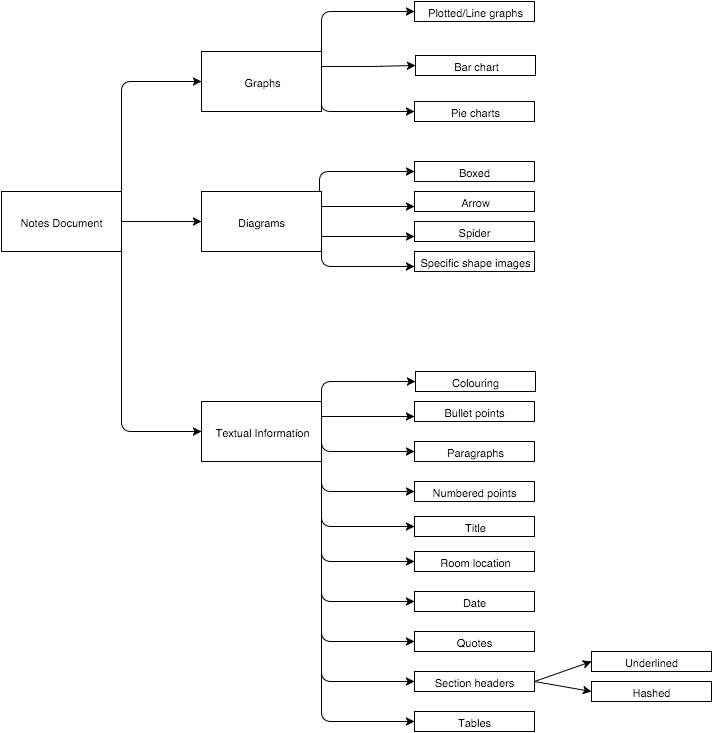
\includegraphics[scale=0.5]{images/taxonomy}
\centering
\caption{A taxonomy showing the structure and classification of different types of notes and what is contained in a note.}
 \label{fig:taxonomyofnotes}
\end{figure}

In Figure \ref{fig:taxonomyofnotes} it shows a taxonomy of the different aspects which may form a part of a note. Textural descriptions form the core content of a note, this is essentially the important aspect that a note-taker is trying to remember and write down. Different note-takers form their notes in different ways, for example the headings may be underlined or hashed - if they were adopting a mark-down style approach. These sections help to show that there's a break in the content, and should be sub-sectioned. Textural points that are short, but important, are often characterised by a colon or a bullet point; these are the most common form of concise note building, in the classification.

Coloured text is often used for a variety of reasons: it stands out on the page and improves memory retention of that text \cite{citeulike:14014177}. Both congruent and incongruent  coloured text helped to increase memory retention of post-graduate learners \cite{Olurinola_Tayo_2015}. With congruent text, Olurinola et al. showed that for 30 students with a 20 word list, a 10.9 mean retention rate was achieved and a 8.1 mean retention rate was achieved for incongruent text. The studies conducted show that coloured items would improve a user's retention rate in a lecture.

Finally, tables help to represent textual content in tabular form - this is often good in notes for comparisons.

Graphs are great visual tools for users to help to convey important textural information easily. Naturally, they have their limitations such as they come in different shapes and sizes, such as a line-graph, pie chart or a bar chart. Coupled with graphs, notes often consist of diagram drawings.  In Figure \ref{fig:taxonomyofnotes}, there are different sections and classifications of a diagram: boxed, arrow etc. Each one has its own purpose and arrowed and box can overlap; UML diagrams are a case of this. Spider diagrams are probably the hardest to represent, due to the varying sizes and whether the user draws circles or clouds. Furthermore, specific shape diagrams are conceptually hard to think about as it depends on the domain in which the user is drawing the note. For example, a person in Biology may draw a stick person, whereas someone in Computer Science may draw a computer.

Identifying a taxonomy of notes is imperative when considering what to parse from a note as it helps to define a domain of possible classifications. By identifying the classifications it will acknowledge what sections can be parsed by a specific technique. For example, textural information and bullet point lists can be parsed via text-recognition however, for diagram recognition that would involve image manipulation.

% Add some more from the stuff Hannah made us write about in the first week.

% Handwriting triaining ?
\subsection{Handwriting recognition}
Analysing a user's handwriting is a complex process and one which requires lots of research. Handwriting recognition has had successes in the past from machine learning techniques, such as neural networks \cite{citeulike:13510433}. Knerr et al. yields a 10\% rejection rate and  a 1\% error rate, with the use of Neural Networks on the U.S. Postal service data collection, showing that handwriting recognition is still very much an active research area, where solutions are still being developed to optimise the correct classifications of text.

Another approach is to analyse handwriting via an OCR (optical character recognition) tool. Rakshit et al. \cite{citeulike:13920972} used the open-source tool, Tesseract \cite{citeulike:14014368} to analyse Roman scripts. The system was trained on handwriting identified from those scripts. Rakshit et al. recorded an 83.5\% accuracy on 1133 characters. It is noted in the paper that ``over-segmentation'' is a problem with the Tesseract engine.

Another issue to overcome when analysing handwriting is disjointed characters; this is where sections of the letter are split off from the main body of the character, for example, the letter i. Rakshit et al. concludes that this is an issue which is ever-present in the Tesseract engine, with around a 53\% misclassification on this character alone.

The problem of handwriting recognition has not been solved - but tools such as Tesseract offers support for improvement in this field. As Rakshit et al., discusses training had to be conducted with Tesseract to ensure that it can identify handwriting successfully. As a result, every implementation of handwriting recognition needs significant amounts of data of varying quality, so that a system can succeed. However, considering Tesseract's high recognition rate of 83.5\% experienced by Rakshit et al., it is a viable option to use for handwriting recognition.

\subsubsection{Tesseract operations}
Tesseract was initially developed by HP, but has now been made into an open-source tool. Ray Smith gives an excellent overview of the Tesseract engine, the following section summaries how Tesseract works. Tesseract uses connected components to identify the outline of characters, these are then collated into blobs. These blobs are then collected into text lines, which are deconstructed into individual words.

The process then goes through a two stage process, of identifying the words first - and the second identifies words which are not well known. Tesseract has the ability to identify textlines from skewed images. Therefore, as long as the image is text, a slight skewing of the image would not affect the ability to identify text. Textlines are found from the blobs, filtered and then sorted aided for tracking. Blobs are then processed in order checking for overlapping coordinates - from which they're either added to a new line, or appended to an existing line.

Smith discusses that the words are then split into characters. Due to handwritten text being varied, as a user would not write uniformly, then chopping is complex.

After the word has been chopped Tesseract needs to segment the character to identify the character. Smith describes that chopping may leave parts of the characters unattached, so an A* algorithm is used to compare different fragments from a graph of chopped characters. These broken characters are then checked against previously trained examples and similar patterns are attempted to be extracted.

The classification is described by Smith as a ``two step process''. Firstly, the character is evaluated and matched against a potential list of characters from previous examples. The second step involves calculating how well that character matches those in the list, the highest match is then selected as the character.

It is important to acknowledge that Smith discusses the implementations of Tesseract as a whole, with results comparable for printed text, not handwritten text - where there is more variation. However, the paper gives a detailed explanation of the complex process of how Tesseract analyses the image, as well as the text.

\subsection{Similar systems}
With note-taking on digital devices becoming more widely available, there has become an influx in note-taking and organisational applications available for users. These are predominately WYSIWYG (what you see is what you get) editors - which allow a great deal of flexibility. When evaluating existing systems three were predominantly used and they were:
\begin{itemize}
  \item OneNote
  \item EverNote
  \item Google Keep
\end{itemize}

\subsubsection{OneNote}
OneNote \cite{citeulike:onenote} is a note-taking and organisational application made by Microsoft, offering the functionality to add text, photos, drag and drop photos onto a plain canvas. In recent times, OneNote has developed functionality to analyse a user's handwriting, from say a stylus, and interpret the text they entered \cite{citeulike:14014236}. In OneNote you can insert a note into a document and then it would interpret the text from the note.

There is a wide range of product support from mobile based applications to web versions of their software. Office Lens \cite{citeulike:14014272} can be used in conjunction with the OneNote to help to take photos and automatically crop the image and then save them to OneNote. This feature is important and should be considered for the \textit{MapMyNotes} application. The process requires the user to sign in with  a Microsoft account. When creating notes, OneNote formats collated notes into a series of ``notebooks''.

One feature which was noted when analysing the system is automatic saving of the note, reducing the need for a user to click save. Additionally, when using OneNote it feels very much like Microsoft Word - with the similar layout that gives most users a similar user experience feel with its intuitive WYSIWYG editor.

\subsubsection{EverNote}
EverNote \cite{citeulike:14014282} is a note-taking and organisional application, it is supported as a web application, bespoke desktop application and a mobile application. EverNote is widely used and provides a wide range of functionality a user would need to digitise their notes.

EverNote have released development articles \cite{citeulike:13988110} stating that OCR recognition on images is possible. This would allow the user to upload an image outputting a list of potential words for each word found in the image. Like OneNote, the notes are collated into Notebooks, offering a WYSIWG editor, giving the user full control of the content that is entered. When uploading an image to the web version it gives the option to edit the PDF and images, however it seems as though an additional application has to be downloaded, specific to the user's platform, to be able to utilise this functionality.

According to the website, it does do OCR recognition, however whilst using the web application there was no information regarding extracting of text from the application. Additionally, there seemed to be no way to save the note to a calendar item - only the option to send via a link.

\subsubsection{Google Keep}
Google Keep \cite{citeulike:14014320} is a note taking application produced by Google with mobile and website support. Google Keep allows a user to attach an image to their note, attempt to extract the text from an image and save this in the body of the note. In addition it allows the user to tag a title and add an associated body.

An important design feature that it does not offer is the support of a WYSIWG editor; a default text box has been preferred, offering a more raw feel to the application. They have the option of a ``remind me'' feature, which will get synced to their calendar as a reminder - but there's no easy way to add it to a calendar event.

Google Keep seems as though it's more suited for TODO lists and jotting down quick notes, rather than an archiving tool suitable for substantial note taking. Nevertheless, the tagging with labels is a nice feature and the filter by image is a smart tool; this only shows notes with specific images. The simplicity of the user interface and the ease in which text can be extract provides a great reference going forward.

\subsubsection{Reflection on the systems}
These three existing products are widely used by the every day note-taker. They have been developed to a high quality and give the user full control of what their notes can consist of. The automatically cropping of an image is an important feature and should be considered  for the application going forward. \textit{MapMyNotes} aims to try and give the user full control of their lecture notes content, so that they can find their notes easily.

\textit{MapMyNotes} intends to differ from EverNote's text extraction by providing a one to one comparison of the text, rather than a list of potential words.

After the analysis of the existing products there are certain aspects which would be regarded as necessary: a simple way to view the notes, a way to filter the notes and a simple UI which feels more like an application rather than a website.


\subsection{Motivation}
The author handwrites his notes during lectures and often are discarded in crowded notebooks until they are needed for an assignment or examination.

A calendar event is already stored for every lecture that the author goes to, so it would be useful if there was a way to associate each of the notes taken to that calendar event. This would ensure that all the information is located in one easy place that can be found again, instead of trawling through lots of paper and trying to find the content again. This would aid in reducing the chances of lost notes from paper slipping out of the notebook or pages being damaged due to rain or creases.

\section{Analysis}
%Taking into account the problem and what you learned from the background work, what was your analysis of the problem? How did your analysis help to decompose the problem into the main tasks that you would undertake? Were there alternative approaches? Why did you choose one approach compared to the alternatives?

%In most cases, the agreed objectives or requirements will be the result of a compromise between what would ideally have been produced and what was felt to be possible in the time available. A discussion of the process of arriving at the final list is usually appropriate.
As the project was originally proposed by Dr Harry Strange, a meeting was arranged to discuss the initial ideas that he wished the application would follow. It was here that it was highlighted that Dr Harry Strange wants to take a photo of his notes, archive them with specific data, make them searchable and integrate them with existing calendar entries he had for a given date.

\subsection{Parsing a note}
In conjunction with the information gathered a taxonomy of notes was collated, helping to deconstruct what a note consists of. Analysing the taxonomy produced a comprehensive breakdown of what could be parsed as text. After seeing that text formed a main component of a note the key efforts of the application would focus on parsing the text. Diagrams, graphs and images were considered when thinking of what should be extracted from an image, however this was placed as a task for the future. This required a task to investigate how to reliably extract the text from an image.

\subsection{An OCR tool}
Handwriting recognition has been an active research project for a while. There could have been the possibility of creating a bespoke handwriting recognition tool, using machine learning techniques, but that would distract from the actual problem which is this available tool to archive notes.

Therefore an OCR tool would have to be chosen to analyse the text. Choosing a sensible OCR tool with good recognition rates would be important - so a task was created to explore and look at possible solutions.

\subsection{What to parse from the note}
From research conducted into Google Keep it was clear that analysing the text would be a great aspect to include in the application. The real question is what should be parsed from the note? By looking at the overall structure of the application and what it entailed then it was agreed to just parse the note's associated meta-data: the title, lecturer, date and module code. Recalling that Google Keep parses all the text and EverNote gives a list of suggested words, it was decided that a tool would be developed to suggest the meta-data but it does not automatically tag the meta-data.

\subsection{Structuring of notes}
In conjunction with analysing what to parse, a sensible structure would have to be applied to notes used in the application. A task to create and find a good set of rules would have to be collated to ensure that notes could be parsed confidently. This reduced the complexity of incorporating natural language processing in the application, which would be implausible to be completed within the timeframe.


\subsection{OCR for the authors handwriting}
After research into OCR technologies, such as Tesseract \cite{citeulike:14014368}, it was established that analysing handwriting is a complicated process. Instead of trying to train it on a lot of dummy data, it would be trained to recognise the author's handwriting. A task was created to train the user's handwriting data and this would run throughout the duration of the project.


\subsection{What platform is most suitable}
During the meeting with Dr Harry Strange one of the core features that was needed was for the application to be accessible regardless of where the user is. After the research was conducted all the aforementioned software tools have a web application version of their system. A mobile application was considered but only one version of the application would be made, either Android or iPhone, therefore preventing other phone users from using the application. A bespoke desktop application was considered for a long time, however, the user would have to ensure infrastructure decisions, such as databases, are correctly set up. As a result a web application was chosen - following research found; the next steps were to consider appropriate tools to use.

\subsection{What should the application do}
From analysing all three of the chosen research systems, it was clearly identifiable that they all have the ability the view all notes, searching, deleting, adding and editing a note. Taking these ideas on-board, they were set as a high-level task and something that the core system \textit{must} do.

Reflecting on the premise of the application, that it was to aid the organisation of lecture notes, it was concluded that the best way to search for notes would be by module code, as most University students would want to find specific module notes. This created the high level task that notes must be searchable by their module code.

\subsection{Calendar integration}
From evaluating the systems it was noticed that there was not a clear way to integrate into a calendar. Reflecting on the conversations with Dr Harry Strange, integrating with the calendar was important for keeping the different systems together. From an AYTM survey, in December 2015, \cite{citeulike:14010520} Google calendar is the most popular calendar application, therefore due to time constraints Google calendar was the choice of integration and other competitors such as Microsoft would not be implemented. This formulates the task of integrating the calendar into the application to save the url of the note to a specific event.

%There should be a clear statement of the objectives of the work, which you will evaluate at the end of the work.
\subsection{Objectives}
As a result of the analysis of the problem, the following high-level requirements were formulated:
\begin{enumerate}
	\item Investigate how to extract handwriting text from an image - this will involve looking into ways OCR tools can interpret handwriting.
	\item Train the OCR to recognise text of the author's handwriting.
	\item Produce a set of a rules which a note must comply to.
	\item Produce a web application to form the core part of the product. This includes allowing a user to upload an image, display the image. Add appropriate tagging to a note such as module code.
	\item The user must be able to search for a given module code, showing the fill list of notes based on the module code entered.
	\item The backend of the application must conduct basic OCR recognition, analysing the first 3 lines of the notes.
	\item The backend must integrate with a calendar to archive the notes away later to be found again.
\end{enumerate}

\subsection{Compromising with objectives}
Some additional compromises were made in-light of the analysis due to the complexity of the tasks at hand.
\begin{itemize}
	\item It would be nice to have image extraction from a note and incorporating a WYSIWG editor into the application, like OneNote.
	\item Full OCR on all the characters. This would then output the text to a blank canvas.
	\item Make the handwriting training generic enough to identify a wide range of users handwriting.
\end{itemize}

It is worth noting down that the project supervisor Dr Hannah Dee felt as though the handwriting training would be too much for the dissertation and should be done as a ``maybe''. After much deliberation it was decided to include it, but as a background process.

\section{Process}
%You need to describe briefly the life cycle model or research method that you used. You do not need to write about all of the different process models that you are aware of. Focus on the process model that you have used. It is possible that you needed to adapt an existing process model to suit your project; clearly identify what you used and how you adapted it for your needs.
Software projects often have a degree of uncertainty with requirements at the beginning, these projects lend themselves to an Agile approach. Whereas more structured applications with requirements which are well known are suited to a plan-driven approach.

For this project there are a lot of tasks which are not 100\% definable at the start of the project. In addition to this certain tasks, such as training the author's handwriting data, can not be truly estimated down to a fixed time. Often new requirements would emerge from weekly meetings and only high level requirements were in-place from the start of the project. As a result, a plan-driven approach such as the Waterfall model would not be appropriate, and an Agile methodology was implemented.

\subsection{Scrum overview}
Scrum \cite{citeulike:14014350} is a methodology used by teams to improve productivity where possible. Due to this being a single person project, a Scrum approach has to be modified. Sprints are set time-boxes where tasks are completed. These vary from one to four weeks in length but a shorter sprint means the developer can act on quicker feedback.

Scrum organises its work into user stories to ensure client valued work is being completed. They are normally collected at the start of the project and put into the backlog, which is a collection of client valued work. At the start of each sprint user stories are selected from the backlog with an estimation on complexity performed. Finally, at the end of the sprint a review and retrospective is conducted to analyse the sprint, identifying what went well and what could be improved.

\subsection{Adapted Scrum}
During the project this methodology was embraced and adapted. A one week long sprint was adopted which coincided with a weekly supervisor meeting. Epics (a high level version of a story) were identified at the start of the project to reflect the work completed in the analysis phase.

The epic was then broken down into user stories. Each user story was formulated as: ``As a \textless role\textgreater I want to \textless feature\textgreater so that \textless resolution\textgreater''. This gave specific client value that was known to have a purpose. Each of these stories were estimated on their complexity and compared to a ``goldilock'' task \footnote{A task which all other tasks are evaluated against.}.

For planning a sprint, the planning poker \cite{citeulike:14014357} technique was adopted; user-stories are estimated on a scale of 1, 2, 3, 5, 8 etc. When a task was estimated about 15 story points, it would be reflected upon to ensure the scope was fully understood - this would be broken down to sub-stories where appropriate.

At the end of a sprint a review and retrospective was conducted in the form of a blog post \cite{citeulike:14014367}, instead of in a team. The retrospective was used to analyse what was achieved in the sprint, what went well and what needed to be improved upon. During this time, pre-planning was conducted to formulate a series of tasks to complete in the next sprint; this was agreed by the customer (Dr Hannah Dee).

Communication with the project supervisor was key to determine what needed to be completed. It was discussed if what was suggested was achievable in that weeks sprint, based on the total story points completed in the previous sprint; if 20 story points were completed in sprint 3 then 20 story points were estimated for sprint 4 - associated user stories were brought forward.

The project was managed on the open source management tool Taiga.io \cite{citeulike:14014360} which was invaluable, and provided built in functionality such as burndown charts per sprint. This shows how well story points are being completed, in the form of velocity, and are used as an analytical tool for how well progression was being made.

Daily stand-ups were informally conducted with a peer. Cut from the usual 15 minutes to around 5 minutes, the conversation helped to identify if there were any issues, what had been completed yesterday and what would be completed that day. This provided a good way to analyse what needed to be achieved and keep in perspective how the sprint was going.

\subsection{Incorporated Extreme Programming}
In tandem with Scrum, Extreme programming \cite{citeulike:13915786} principles were integrated into the development process; merciless refactoring, continuous integration and test-driven development were borrowed from its principles.

\subsubsection{Test-driven development}
Test-driven development (TDD) is the process of writing tests prior to the implemented code. This allows the developer to think about the design prior to its implementation and can form part of the documentation \cite{citeulike:14014361}. This was implemented throughout the project, with both unit and acceptance tests being written before the code implementation.

TDD follows three cycles: red, green, refactor. Initially the test fails, then it passes then refactoring is performed to keep the simplest system.

\subsubsection{Continuous Integration}
Continuous Integration tools were a core part of the process in this project. Typically used to ensure that code is checked into a repository it was used to ensure that the application could be built in an isolated environment and pass all the tests.

\subsubsection{CRC cards}
Class, responsibilities and collaboration (CRC) cards \cite{citeulike:13398676} were used during the design section to consider how different classes were to be created and the responsibilities they share. This principle from Extreme Programming helped to keep the design simple and not convoluted.
